% !TeX root = ../main.tex

\chapter{绪论}

\section{网格切割}

曲面网格,又经常被简称为网格,是曲面的分片线性表示,是计算机图形学的基石。栩栩如生的 3D 游戏和 CG 电影,以及在工程上广泛应用的有限元物理仿真方法,其背后离不开高精度的网格。

为了让网格本身适应各种场景下的应用,或是为了获得某些网格的变体,研究者们发明了许多网格的处理和变换过程,这些过程又被称为网格的几何处理。

参数化,如图 \ref{fig:texmapping} 所示,即寻找网格到另一个网格或平面的映射,并且使其满足一些特定的要求,是典型的几何处理问题之一\cite{Floater1997}。以纹理映射要求下的参数化应用为例,用户希望获得一个网格到 $ [0, 1] \times [0, 1] $ 的映射,并且将模型的颜色、法线细节等绘制于这个映射到的平面区域中,从而在节约计算资源的同时增强模型的真实感和表现力\cite{wikitexturemapping}。

\begin{figure}[h]
    \centering
    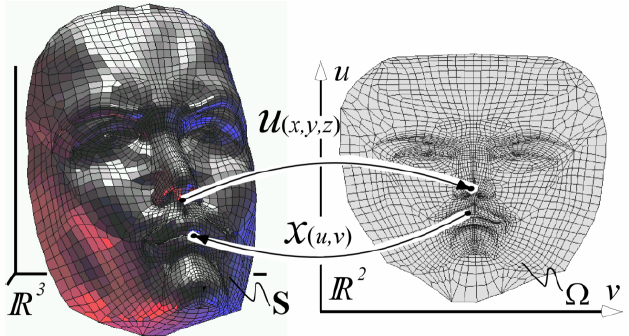
\includegraphics[width=0.7\textwidth]{para.png}
    \caption{参数化示意图,两个方向的映射分别用 $u$ 和 $x$ 表示}
    \label{fig:texmapping}
    \note{图片源自互联网}
\end{figure}

曲面网格的许多几何处理过程,如参数化,都依赖网格的拓扑信息。在某些场景下,我们希望能将带有复杂拓扑的网格,在保持几何信息近似不变的情形下变为圆盘拓扑,这就是曲面的切割问题。

以纹理映射为例,我们希望获得一个网格曲面到 $ [0, 1] \times [0, 1] $ 的双射,而此映射存在的必要条件是两个拓扑空间同胚。这时,唯一的方法就是将该网格曲面切割,使结果拓扑同胚于圆盘。\cite{Erickson2002} 不过,我们注意到对个别情况来说,纹理会被嵌入到二维球 $ S^2 $ 上,这时候我们需要同胚于球面的网格\cite{Haker2000}。

对于不同的几何处理过程,对三维网格的要求各不相同,切割时应加以考虑。对于纹理映射来说,一个常见的要求是寻找使参数化后三角形形变最小的切割方案\cite{Floater1997}\cite{Gu2002}。另一个常见的要求是令割线尽可能短,这在提高纹理映射后图集生成的空间利用率上很有帮助\cite{atlasgen}。

\section{相关工作}

由于网格切割在计算机图形学中的重要地位,切割和割线优化问题被研究者们广泛研究。寻找可以将网格切割为圆盘的割线是快速的,\citet{Dey1995} 说明只需要对对偶图进行广度优先搜索,就可以在 $ O(n) $ 的时间复杂度下得到将网格切割为圆盘拓扑的割线;\citet{Gu2002} 中给出了一个实现上快速且简便的网格切割算法;\citet{DeVerdiere2005} 给出了基于同伦等价的最短圈集合的网格切割算法。

但是,优化割线长度是比较困难的。\citet{Erickson2002} 证明了,对于二维流形网格来说,计算其总长度或总段数意义下的最短割线是 NP-Hard 问题,并且提出了 $ O(g^2 n \log n) $ 时间复杂度的最小切割图近似算法;\citet{oncomputinghantun} 定义了柄圈,并给出了计算曲面上较短柄圈的实现\cite{Dey2013}\cite{Dey2008};\citet{Chai2018}指出柄圈可能是优化割线长度的曲面切割问题的好的启发。

对于网格参数化过程而言,除了割缝长度外还存在其它优化目标。传统上来说,参数化由两个问题构成:寻找割缝切割曲面\cite{qdmeshseg}\cite{KhodakovskyLS03}和最小化扭曲\cite{Desbrun2002}\cite{KhodakovskyLS03}。早期的工作大多只考虑了一个问题,或者是将两个问题顺序优化。之后,也有同时考虑两方面问题的工作出现\cite{Li2018}。

除此之外,许多工作也侧重于割缝生成的其它方面。\citet{Poranne2017} 提供了交互式的割缝生成和参数化展开框架,满足了参数化时低扭曲和对割缝位置的两方面要求;\citet{wysiwyg} 实现了改进的 ABF++ 方法来实现交互式割缝生成和参数化迭代;\citet{teimury2020graphseam} 基于图神经网络 (GNN) 实现了支持语义的割缝生成系统,从而将扭曲和割缝长度之外的因素考虑进来。

\section{本文内容}

本文首先介绍了曲面和曲面网格的定义,并给出了给定割线集情况下的基于 Euler 图的局域网格切割基本方法。之后,本文给出了来自 Geometry Images 中的简单网格切割算法实例。
  
一些几何处理问题,如参数化和图集生成,需要寻找长度尽可能短的割线集。本文回顾了代数拓扑中单纯同调论的基本知识,总结了割线集优化的相关结果,并且复现了计算在权重函数最短意义下的 $ \mathbb{Z}_2 $ 域一维同调群基向量组的工作,此工作可以为计算基于把手链的闭曲面网格切割算法提供帮助。之后,本文介绍了柄圈的形式化定义和基本计算方法,并给出了基于 TetGen 网格剖分工具的实验性实现。

最后,本文给出了部分算法的实现。

% \subsection{二级节标题}

% \subsubsection{三级节标题}

% \paragraph{四级节标题}

% \subparagraph{五级节标题}

% 本模板 \pkg{ustcthesis} 是中国科学技术大学本科生和研究生学位论文的 \LaTeX{}
% 模板, 按照《\href{http://gradschool.ustc.edu.cn/static/oldsite/ylb/material/xw/wdxz/32.pdf}
% {中国科学技术大学研究生学位论文撰写手册}》(以下简称《撰写手册》)和
% 《\href{https://www.teach.ustc.edu.cn/notice/notice-teaching/11530.html}
% {关于本科毕业论文(设计)格式和统一封面的通知}》的要求编写。

% Lorem ipsum dolor sit amet, consectetur adipiscing elit, sed do eiusmod tempor
% incididunt ut labore et dolore magna aliqua.
% Ut enim ad minim veniam, quis nostrud exercitation ullamco laboris nisi ut
% aliquip ex ea commodo consequat.
% Duis aute irure dolor in reprehenderit in voluptate velit esse cillum dolore eu
% fugiat nulla pariatur.
% Excepteur sint occaecat cupidatat non proident, sunt in culpa qui officia
% deserunt mollit anim id est laborum.



% \section{脚注}

% Lorem ipsum dolor sit amet, consectetur adipiscing elit, sed do eiusmod tempor
% incididunt ut labore et dolore magna aliqua.
% \footnote{Ut enim ad minim veniam, quis nostrud exercitation ullamco laboris
%   nisi ut aliquip ex ea commodo consequat.
%   Duis aute irure dolor in reprehenderit in voluptate velit esse cillum dolore
%   eu fugiat nulla pariatur.}
